\documentclass{standalone}
\usepackage{tikz}
\begin{document}
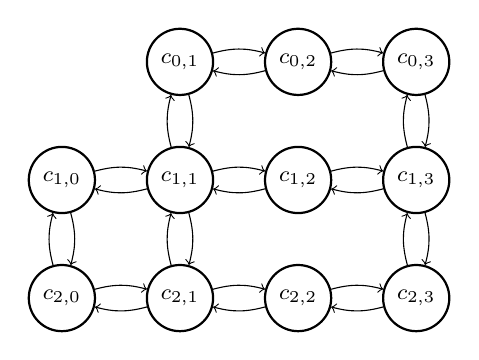
\begin{tikzpicture}[
  node distance=1.5cm,
  every node/.style={circle, draw,thick, minimum size=0.6cm},
  every edge/.style={->, thick}
  ]

  % Define nodes
  \node (00) at (0,0) {{\footnotesize $c_{2,0}$}};
  \node (10) at (1.5,0) {{\footnotesize $c_{2,1}$}};
  \node (20) at (3,0) {{\footnotesize $c_{2,2}$}};
  \node (30) at (4.5,0) {{\footnotesize $c_{2,3}$}};

  \node (01) at (0,1.5) {{\footnotesize $c_{1,0}$}};
  \node (11) at (1.5,1.5) {{\footnotesize $c_{1,1}$}};
  \node (21) at (3,1.5) {{\footnotesize $c_{1,2}$}};
  \node (31) at (4.5,1.5) {{\footnotesize $c_{1,3}$}};

  \node (12) at (1.5,3) {{\footnotesize $c_{0,1}$}};
  \node (22) at (3,3) {{\footnotesize $c_{0,2}$}};
  \node (32) at (4.5,3) {{\footnotesize $c_{0,3}$}};

  % Horizontal edges (bidirectional pairs)
  % Bottom row
  \draw (00) [->] to[bend left=15] (10);
  \draw (10) [->] to[bend left=15] (00);
  \draw (10) [->] to[bend left=15] (20);
  \draw (20) [->] to[bend left=15] (10);
  \draw (20) [->] to[bend left=15] (30);
  \draw (30) [->] to[bend left=15] (20);

  % Middle row
  \draw (01) [->] to[bend left=15] (11);
  \draw (11) [->] to[bend left=15] (01);
  \draw (11) [->] to[bend left=15] (21);
  \draw (21) [->] to[bend left=15] (11);
  \draw (21) [->] to[bend left=15] (31);
  \draw (31) [->] to[bend left=15] (21);

  % Top row
  \draw (12) [->] to[bend left=15] (22);
  \draw (22) [->] to[bend left=15] (12);
  \draw (22) [->] to[bend left=15] (32);
  \draw (32) [->] to[bend left=15] (22);

  % Vertical edges (bidirectional pairs)
  % (0,0) and (0,1)
  \draw (00) [->] to[bend left=15] (01);
  \draw (01) [->] to[bend left=15] (00);

  % (1,0) and (1,1)
  \draw (10) [->] to[bend left=15] (11);
  \draw (11) [->] to[bend left=15] (10);

  % (1,1) and (1,2)
  \draw (11) [->] to[bend left=15] (12);
  \draw (12) [->] to[bend left=15] (11);

  % (3,0) and (3,1)
  \draw (30) [->] to[bend left=15] (31);
  \draw (31) [->] to[bend left=15] (30);

  % (3,1) and (3,2)
  \draw (31) [->] to[bend left=15] (32);
  \draw (32) [->] to[bend left=15] (31);

  % % Annotation on edge for p and q functions
  % % \draw (1.65,0.75) [-] to (2.25,-0.75)
  % % node[draw=none, align=left] (100) at (2.25,-1.2) {{\footnotesize $p(e) = \{s,e\}$} \\ {\footnotesize $q(e) = s$}};
  % \draw (1.25,0.75) [-] to (0.25,2.8)
  % node[draw=none, align=left] (100) at (-1,3) {{\footnotesize $p((c_{1,2},c_{1,1})) = \{e\}$}};
  % \draw (1,0.5) [-] to (0.25,2.4)
  % node[draw=none, align=left] (100) at (-1,2.5) {{\footnotesize $q((c_{0,2},c_{1,2})) = e$}};

\end{tikzpicture}
\end{document}
%
%%% Local Variables:
%%% mode: LaTeX
%%% TeX-master: t
%%% End:
